%!TEX root = ../template.tex
%%%%%%%%%%%%%%%%%%%%%%%%%%%%%%%%%%%%%%%%%%%%%%%%%%%%%%%%%%%%%%%%%%%
%% chapter1.tex
%% NOVA thesis document file
%%
%% Chapter with introduction
%%%%%%%%%%%%%%%%%%%%%%%%%%%%%%%%%%%%%%%%%%%%%%%%%%%%%%%%%%%%%%%%%%%

\typeout{NT FILE chapter1.tex}%

\chapter{Introdução}
\label{cha:introduction}

\prependtographicspath{{Chapters/Figures/Covers/}}

% epigraph configuration
\epigraphfontsize{\small\itshape}
\setlength\epigraphwidth{12.5cm}
\setlength\epigraphrule{0pt}

\noindent Este capítulo tem como objetivo introduzir o tema da dissertação a ser desenvolvida. 
É apresentada a motivação para a realização do projeto, o contexto em que o problema abordado se insere e os objetivos a serem alcançados. 

\section{Motivação}
\label{sec:motivation}
Nos últimos anos, os Large Language Models (LLMs) têm revolucionado a área da inteligência artificial, alterando drasticamente a forma como interagimos com máquinas.
Estes modelos, treinados a partir de uma vasta quantidade de dados, destacam-se pela sua capacidade para compreender, interpretar e gerar texto em linguagem natural, permitindo interações mais fluidas e próximas do diálogo humano.
Esta inovação permite uma melhoria no serviço em diversas áreas, como o atendimento ao cliente, automação de processos e suporte técnico. 

Simultaneamente, a sociedade tem exigido cada vez mais soluções tecnológicas que melhorem a eficiência, acessibilidade e conveniência de serviços. 
Serviços como a renovação do passaporte, que antes exigiam deslocações a instalações físicas, o que causava um transtorno para o cidadão que tinha de fazer esse deslocamento e, muitas vezes, gastar tempo em filas de espera, estão rapidamente a ser substituídos por opções remotas, acessíveis a qualquer momento e lugar.

As LLMs representam um avanço face aos chatbots tradicionais, estes que têm uma abordgem mais rígida e incapaz de lidar com a complexidade e ambiguidade, algo característico da comunicação humana. 
A utilização das LLMs oferece flexibilidade, adaptabilidade e a capacidade de aprender continuamente, o que faz com que esta seja uma opção ideal para casos de apoio ao cliente.

Com estes avanços, é possível melhorar

\section{Contexto}
\label{sec:context}

\section{Objetivos}
\label{sec:objetivos}

\section{Organização}
\label{sec:organization}

O documento está organizado nos seguintes capítulos:
\begin{enumerate}
  \item \textbf{Introdução - } Neste capítulo, é definida a motivação e contexto da dissertação, bem como os seus objetivos.
  \item \textbf{Estado da Arte - } Neste capítulo, é apresentado o estado da arte. São estudadas soluções semelhantes já existentes e apresentados conceitos importantes para a compreensão desta dissertação.
  \item \textbf{Tecnologias - } Neste capítulo, são apresentadas ferramentas estudadas para a elaboração da solução.   
  \item \textbf{Solução Proposta - } Neste capítulo, é apresentada a solução (descrição, tecnologias a usar, plano de trabalhos, requisitos da solução, US?).
\end{enumerate}

The \gls{novathesis} template was born in~1996, and what you see now accumulates to many many hundreds (thousands?!) of working hours, unpaid and stolen from family and friends.  This work is available to the community under the \href{LaTeX project public license}{\LaTeX\ Project Public License v1.3c}, which means you are entitled to use it for free and change it at your will.  However, if you decide to use this template to write your thesis/dissertation, \textbf{be fair to the developers} and:
\begin{enumerate}
  \item \ntindex[novathesis!Citation]{} Cite the \gls{novathesis} manual~\cite{novathesis-manual} in a place of your choice (e.g., in the \emph{Acknowledgments}) of your thesis/dissertation with “\verb!\cite{novathesis-manual}!” .  If you cite it this way, the correct entry will be added automatically to your bibliography (no need to worry with the necessary BibTeX entry, as it will be added automatically);
  \item Go to the
\href{https://github.com/joaomlourenco/novathesis}{\ntindex[GitHub!project web page]{project web page} in GitHub} and give the project a \ntindex[GitHub!stars]{star} (marked with a red ellipse at the top-right in Figure~\ref{fig:github}); and
  \item Make a \ntindex[donations]{donation} by visiting the \gls{novathesis} project page and clicking in the button marked with a green ellipse at the top-center in Figure~\ref{fig:github}).  Alternatively, just click \href{https://www.paypal.com/donate/?hosted_button_id=8WA8FRVMB78W8}{\fcolorbox{DarkGreen}{gray!15}{\textbf{~HERE~}}} and your browser will be directed to the right page.
\end{enumerate}

\begin{figure}[htbp]
    \centering
    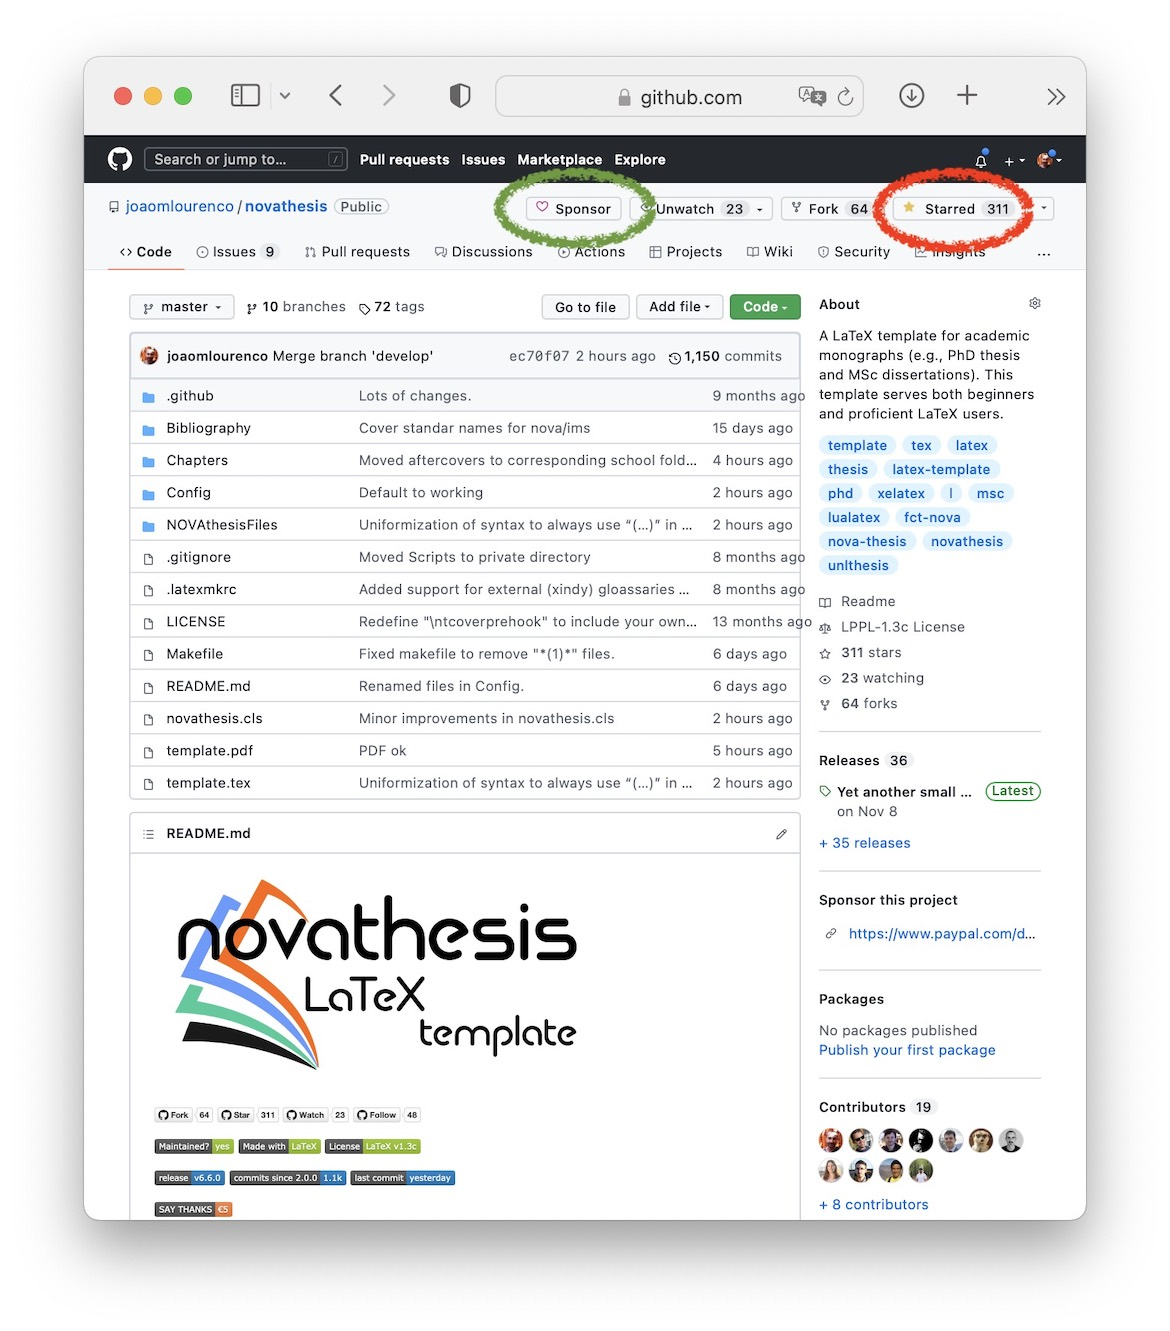
\includegraphics[width=0.5\linewidth]{github1}
    \caption{The \gls{novathesis} project web page in GitHub.}
    \label{fig:github}
\end{figure}